\documentclass{article}
    % General document formatting
    \usepackage[margin=0.7in]{geometry}
    \usepackage[parfill]{parskip}
    \usepackage[utf8]{inputenc}
    
    % Related to math
    \usepackage{amsmath,amssymb,amsfonts,amsthm,mathtools}
	% for the figures
	\usepackage{graphicx}
	%
	\usepackage{xspace}

	\usepackage{algorithm}
	\usepackage{algpseudocode}
    

\newcommand{\fullsys}{Coalesced Intermittent Sensor\xspace}
\newcommand{\sys}{CIS\xspace}
\title{Coalesced Intermittent Sensor: Patent Description}

\begin{document}
\maketitle

\begin{figure}[!h]
		\centering
		\includegraphics[]{figures/cis}
		\caption{A Coalesced Intermittent Sensor (CIS) is a group of energy-harvesting intermittent sensors (EHSs). Its uptime is characterized by a uniform distribution of its EHSs uptimes.}
		\label{fig:cis}
\end{figure}
\section*{Coalesced Intermittent Sensor}
A Coalesced Intermittent Sensor (CIS) is defined as the abstraction of a group of energy-harvesting intermittent sensors (EHSs) providing the collective sense of being always on (Figure~\ref{fig:cis}).

\section*{Estimating the number of active intermittent sensors}
%
\begin{figure}[t]
		\centering
		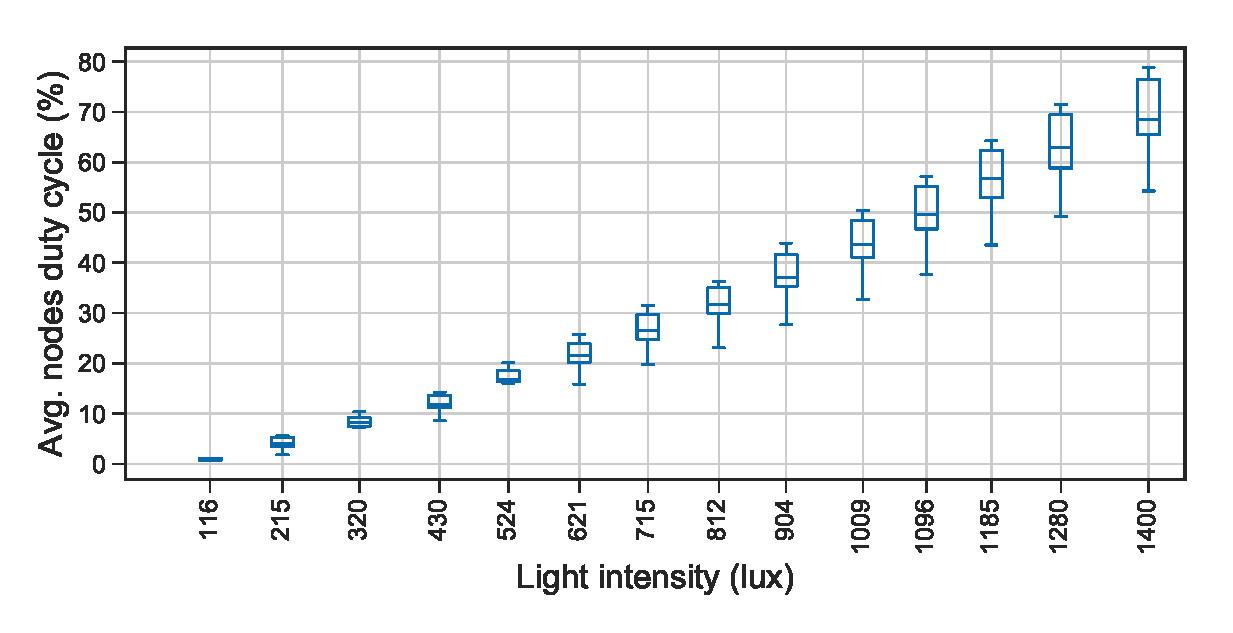
\includegraphics[width=.5\textwidth]{figures/cis_dutyCycle}
		\caption{The average duty cycles of eight intermittently powered nodes for different light intensity. In general, an individual node's duty cycle is a good indicator of the average duty cycle of its \sys.}
		\label{fig:cis_nodes_dutyCycle}
\end{figure} 
%

\begin{algorithm}[t]
	\caption{algorithm}{off-time estimation}
    \label{algo:offTime}
    \small
    \begin{algorithmic}[1]
		\State \Call{$f_\text{reboot}$}{$u$} $= u{+}{+}$ \Comment{power reboot counter}
			\State $i \leftarrow $ \Call{$f_\text{reboot}$}{$i$} \Comment{$i$ is a persistent variable} \label{lin:i}
		\State $E_\text{buf}$ \Comment{Size of energy buffer}
			\State $t_a$ \Comment{time of discharging $E_\text{buf}$ at load $a$, no harvesting}\label{lin:ta}
		\State$ t_{i} \leftarrow x $ \Comment{timing every $x$ power cycles}
		%
		\If{$(i\mod t_{i})=0$}
		    \State $i=0$
			\State \Call{$f_\text{load}$}{$a$} \Comment{set node load to $a$ } \label{lin:fixedLoad}
			\State \label{lin:ontime} $t_\text{on} \leftarrow$ \Call{$t_\text{pers}$}{\null} \Comment{persistent infinite loop}\label{lin:ton}
		\EndIf
		\If{$i=1$}
			\State \label{lin:deltat}$\Delta{t} = t_\text{on}-t_a$  \Comment{time difference due to charging} \label{lin:td}
			\State \label{lin:ehar}$E_\text{har} \leftarrow (E_\text{buf}\div t_a)\times\Delta{t}$ \Comment{harvested energy}
			\State $P_\text{in} \leftarrow E_\text{har}\div{t_\text{on}}$ \Comment{incoming power} \label{lin:pin}
			\State \label{lin:offtime}$t_\text{off} \leftarrow E_\text{buf}\div P_\text{in}$ 
		\EndIf
	\end{algorithmic}
\end{algorithm}

\begin{figure}
		\centering
		\includegraphics[]{figures/softwareClock}
		\caption{an energy buffer discharge time when a sensor node harvests energy while executing and when it does not. Ehar is the amount of energy harvested during the discharge time of the device (when the device is operating).}
		\label{fig:softwareClock}

\end{figure}

In order for an energy-harvesting intermittent node to estimate the number of its active neighbors, it needs three ingredients: (i) the total number of its neighbors, (ii) the on/off cycles of its neighbors, and (iii) how the awake times of the EHSs are distributed. 

The first ingredient, we assume to be provided before the deployment time. For the second ingredient, we assume that the sensor nodes are equipped with the same energy harvester, including the buffer size, and they are in a close proximity (Figure~\ref{fig:cis}). Based on these assumptions, a node can measure its own power cycle (on/off cycle) and use it to estimate neighbors' power cycles. Figure~\ref{fig:cis_nodes_dutyCycle} shows eight nodes duty cycles under different light intensities. In general, we can conclude that a node duty cycle is a good metric to estimate the duty cycle of other nodes. But, \emph{how a EH sensor can determine its own on/off cycle (or power cycle)?}
To calculate to off-time of an EHS, the incoming power (or charging rate) need to be measured and the size of the buffer need to be known. The buffer size is fixed and can be pre-loaded to the device memory.
To measure the incoming power, we need to determine the amount of energy harvested while the device is executing, $E_\text{har}$, and measure the time of harvesting (Figure~\ref{fig:softwareClock}).
$E_\text{har}$ can be determined through measuring the time in two different scenarios on a fixed load. 
First, we need to  measure the time needed to discharge the energy buffer (after being fully charged) while harvesting is disabled $t_\text{a}$ (Line~\ref{lin:ta}, Algorithm~\ref{algo:offTime}). $t_\text{a}$ is a constant value that needs to be measure or calculated only once and saved into the device memory. 
To measure the time needed to discharge the buffer while the device is harvesting, $t_\text{on}$, a persistent timer is needed (Line~\ref{lin:ton}), as the micro-controller built-in timers are volatile: meaning, they lose their values on a power failure. A simple way to have a persistent timer is to use a software non-volatile counter. 

The power consumption during time measurement should be fixed to establish a linear relationship between time and energy consumption (Line~\ref{lin:fixedLoad}).  
Using the obtained values an EHS can run Lines~\ref{lin:td}-\ref{lin:pin} of Algorithm~\ref{algo:offTime} to calculate the off-time. 

Since, calculating the off-time requires constant load, the sensor cannot run arbitrary code during time measurement. Therefore, the sensor need to sacrifice a certain percentage of its power-ups for time measurement, Line~\ref{lin:i}-\ref{lin:ton}. Once the on-time and off-time are found the power cycle is determined. 


For the third ingredient, we, ideally, would like to EHSs' awake times to be perfectly aligned next to each other, achieving maximum availability. However, to approximate maximum span a form of communication for coordination is needed. Communication for coordination may introduce significant overhead and further tighten the energy budget for other duties. 
Alternatively, a probabilistic approach can be applied. 
Instead of trying to specify the probability distribution of the awake times of EHSs, we would like to enforce them to be uniformly distributed.  
The uniform distribution leads to maximum randomness which, in turn, leads to maximum awake time probabilistic spreading. In other words, we would like to break any correlation resulting from drawing energy from the same source, having the same characteristics, and/or being in a close proximate.   

\begin{figure}[t]
		\centering
		\includegraphics[width=.5\columnwidth]{figures/cisOntime}
		\caption{A \fullsys's availability is the emerging collective on-time of its intermittent nodes' on-times. The difference between the power cycles leads to a constant relative shift between the nodes duty cycles. This, in turn, causes their on-times to be uniformly distributed on the overall power cycle. The red bars indicate a minimum \sys time span---\sys's nodes are overlapping---whereas the green bars show the maximum time span of the \sys.}
		\label{fig:cisOntime}
\end{figure} 

Uniform distribution can be approximated by ensuring that the power cycles of the EHSs are slightly different. 
The $\Delta{t}$ difference between the length of the on/off cycles will cause them to shift relative to each other after each cycle. This dynamic behavior makes the awake times of the EHSs to be uniformly distributed overtime.
Figure~\ref{fig:cisOntime} illustrates the scenario of two intermittent nodes with different power cycles. Node 1 has a power cycle of 6 units of time and an on/off cycle of $\frac{1}{3}$. Node 2 has a power cycle of 5 units of time and an on/off cycle of $\frac{1}{5}$. Following the time axis from the left, we can see that the position of the on-time of Node 2 is shifted by 1 unit of time after each power cycle of Node 2. This implies that the on-times of the two nodes are $\frac{1}{3}$ of the time cluster together and $\frac{2}{3}$ of the time they are apart. If we extend the previous scenario to three or more nodes then the on-time of the resulting \sys can be described with the following formula,
\begin{equation}
	t_\text{on}(N) = t_\text{on}(N-1) + \frac{t_\text{off}(N-1)}{t_\text{off}(N-1)+t_\text{on}(N-1)} \times t_\text{on}(1),
		\label{eq:cisModel}
\end{equation}
where $N \in \mathbb{N}$ and  $t_\text{on}(N)$ is the on-time of a \sys with $N$ intermittent nodes. For the initial case where $N=1$ we define $t_\text{on}(0)\coloneqq 0$ and $t_\text{off}(0) \coloneqq 1$.


\section*{Coalesced Intermittent Sensors Network}
[This section is added to relect on the ``Field of the invention'' paragraph]
Figure~\ref{fig:cis_net} shows an imaginary wireless network of \sys{}s. Message passing between intermittent EHSs is unreliable as they are available only a fraction of the time. However, massage passing between \sys{}s is more reliable as their availability can be made to approach continuous time. 

\begin{figure}[t]
		\centering
		\includegraphics[width=.5\columnwidth]{figures/cis_net}
		\caption{Each node of \fullsys Network is a group of Energy-harvesting Intermittent Sensors (EHSs).}
		\label{fig:cis_net}
\end{figure} 


















\end{document}
